\documentclass{article}
\usepackage[utf8]{inputenc}
\usepackage[UKenglish]{babel}
\usepackage[UKenglish]{isodate}
\usepackage{fullpage}
\usepackage[affil-it]{authblk}
\usepackage{pdfpages}
\usepackage{amsmath}
\usepackage{amsfonts}
\usepackage[capitalise]{cleveref}
\usepackage{mathrsfs}
\usepackage{complexity}
\usepackage{siunitx}
\usepackage{tikz}
\usepackage{subcaption}

\usetikzlibrary{arrows}
\usetikzlibrary{arrows.meta}
\usetikzlibrary{calc}
\usetikzlibrary{positioning}
\usetikzlibrary{shapes}

\title{Probabilistic Inference in Graphical and Relational Models}
\author{Paulius Dilkas \\[1ex] {\small Supervisors: Mr Vaishak Belle and Dr Ron
    Petrick}}
\affil{School of Informatics, University of Edinburgh}

\definecolor{first}{HTML}{1b9e77}
\definecolor{second}{HTML}{d95f02}
\definecolor{third}{HTML}{7570b3}
\definecolor{fourth}{HTML}{e7298a}
\definecolor{fifth}{HTML}{66a61e}

\begin{document}
\maketitle

\section{Introduction}

This document has four sections and four appendices:
\begin{itemize}
\item \Cref{sec:background} contains background information on various
  representations of probability distributions, their applications, and
  inference algorithms.
\item \Cref{sec:progress} describes the research progress made this academic
  year.
\item \Cref{sec:future} provides a plan for the rest of my degree.
\item \Cref{app:cp,app:uai,app:sat} contain papers either published or submitted
  since last year's review.
\item And last year's review itself is included in \cref{app:previous}.
\end{itemize}

\section{Background} \label{sec:background}
% TODO: 2-3 pages. and introduce Section 2.

\subsection{Representations of Probability Distributions}
% ILP \cite{DBLP:journals/ngc/Muggleton91}, PILP \cite{DBLP:conf/ilp/2008p}

Perhaps the best-known representations of probability distributions are
probabilistic graphical models (PGMs), i.e., graphs with vertices that
correspond to random variables. The graph can either be directed (as in Bayesian
networks \cite{DBLP:books/daglib/0066829}) or undirected (as in Markov random
fields \cite{spitzer1971markov}). Both PGMs have been extended to support
additional structure: relational Bayesian networks \cite{DBLP:conf/uai/Jaeger97}
can compactly describe a probability distribution over a relational structure,
and Markov logic networks (MLNs) \cite{DBLP:journals/ml/RichardsonD06} extend
Markov random fields with support for first-order logic. In fact, efforts to
unify probability and logic have a history going back to mid-1980s
\cite{DBLP:journals/ndjfl/Hailperin84,DBLP:journals/ai/Nilsson86}.

TODO: two more references to mention: \cite{DBLP:series/synthesis/2016Raedt} and
\cite{DBLP:series/sci/BrazAR08}

Augmenting a programming language with probabilities is another common approach
to conveniently and compactly represent a probability distribution. Logic
programming languages in particular have been frequently used for this purpose,
examples of which include earlier languages such as independent choice logic
\cite{DBLP:journals/ai/Poole97} and PRISM \cite{DBLP:conf/ijcai/SatoK97} as well
as more recent ones such as ProbLog \cite{DBLP:conf/ijcai/RaedtKT07} and
CP-logic \cite{DBLP:journals/tplp/VennekensDB09}. Functional and imperative
programming languages have also seen some use. Probabilistic semantics in these
languages typically rely on two constructs: the ability to draw random values
from probability distributions and the ability to condition a program on
observations \cite{DBLP:conf/icse/GordonHNR14}. Examples of such languages
include functional languages such as Church \cite{DBLP:conf/uai/GoodmanMRBT08}
and imperative languages like BLOG \cite{DBLP:conf/ijcai/MilchMRSOK05}.

Probabilities (more specifically, transition probabilities) are also central to
Markov decision processes \cite{bellman1957markovian} and partially observable
Markov decision processes \cite{aastrom1965optimal}, and so are heavily used in
planning languages such as relational dynamic influence diagram language (RDDL)
\cite{sanner2010relational} and probabilistic model checkers such as PRISM
\cite{DBLP:conf/cav/KwiatkowskaNP11}. Finally, probabilities are even used in
databases as a way to represent uncertainty about the correctness or accuracy of
the data \cite{DBLP:series/synthesis/2011Suciu}.

\paragraph{Applications.}
Probabilistic models have been successfully applied to many domains. Here we
primarily focus on applications in life sciences, natural language processing,
and robotics. Statistical relational models have been widely used to analyse
genetic \cite{DBLP:journals/nar/MaeyerWRRM15,DBLP:journals/jcb/SakhanenkoG12}
and medical \cite{DBLP:conf/iaai/NatarajanKIJC13} data and in particular have
been successfully applied to breast cancer diagnosis and decision support
\cite{DBLP:conf/ilp/Corte-RealD017,DBLP:conf/pkdd/NassifKBPSC13}. In natural
language processing, probabilistic models have been used to extract events
\cite{DBLP:conf/emnlp/VenugopalCGN14} and knowledge
\cite{DBLP:conf/naacl/PoonV10} from text, classify sentences
\cite{DBLP:conf/emnlp/VerbekeAMFDR12}, efficiently model a language
\cite{DBLP:conf/icml/JerniteRS15}, solve textbook probability problems
\cite{DBLP:conf/ijcai/DriesKDBR17}, and form beliefs from reading various web
pages \cite{DBLP:conf/aaai/CarlsonBKSHM10}. Representations such as MLNs and
ProbLog have also been used in robotics to model object affordances
\cite{DBLP:conf/icra/MoldovanMOSR12,DBLP:conf/iros/MoldovanR14,DBLP:conf/ilp/MoldovanORMS11},
enable a robot control system to deal with ambiguities in natural language
instructions \cite{DBLP:journals/ras/BeetzJMT10}, or more generally as the
robot's probabilistic knowledge representation system
\cite{DBLP:conf/icra/JainMB09}. Finally, probabilistic models have also been
used for many other tasks such as planning under uncertainty (MDPs)
\cite{DBLP:journals/jair/BoutilierDH99}, knowledge base construction (MLNs)
\cite{DBLP:journals/ijswis/NiuZRS12}, stream mining
\cite{DBLP:conf/icdm/ChandraSKTA14}, predicting the remaining useful life of a
hardware component \cite{vlasselaer2012statistical}, recommendation systems
\cite{DBLP:journals/corr/YangKAGN16}, and criminal activity prediction
\cite{DBLP:conf/sdm/DelaneyFCWJ10}. The reader can mind many more examples in a
book by De Raedt et al. \cite{DBLP:series/synthesis/2016Raedt}.

\subsection{Probabilistic Inference}
% TODO: emphasise definitions

The problem of computing some probability from a given representation of a
probability distribution can be seen as a version of a more general problem
known as SumProd
\cite{DBLP:journals/jair/BacchusDP09,DBLP:journals/ai/Dechter99}. It is
characterised by a set of discrete variables and a set of functions from some
subsets of the variables to a commutative semiring. SumProd then asks to compute
the sum over all values of all variables of the product of all functions. Many
problems such as SAT, constraint satisfaction, model counting, and most probable
explanation can be describe as variations of SumProd
\cite{DBLP:journals/jair/BacchusDP09,DBLP:journals/ijar/BelleR20,DBLP:journals/ai/Dechter99,DBLP:journals/japll/KimmigBR17}.
It is often convenient to consider two graphs associated with each instance of
SumProd. Its canonical hypergraph has variables as vertices and function domains
as edges, and its primal graph (also known as the Gaifman graph and by many
other names) is the simple graph with variables as vertices and an edge
between two variables if there is a function that depends on both of them.

A number of algorithms for probabilistic inference have been proposed.
\begin{itemize}
\item Variable elimination \cite{DBLP:journals/ai/Dechter99} works by
  nondeterministically choosing an ordering of variables and `summing out' each
  variable in the chosen order. The well-known
  Davis-Putnam algorithm \cite{DBLP:journals/jacm/DavisP60} for SAT is an
  example of variable elimination \cite{DBLP:journals/jair/BacchusDP09}.
\item Recursive conditioning \cite{DBLP:journals/ai/Darwiche01} is a
  divide-and-conquer algorithm that relies on a branch decomposition of the
  hypergraph to initialise variables in such a way so as to split the problem
  into multiple smaller problems that can be solved independently. AND/OR search
  \cite{DBLP:journals/ai/DechterM07,nilsson1980principles} is a similar
  technique that utilises pseudo trees of the primal graph instead of branch
  decompositions.
\item Belief propagation (also known as message passing)
  \cite{DBLP:conf/aaai/Pearl82} is an approximation algorithm that converges to
  the exact answer when the primal graph is a tree or a polytree (i.e., a
  directed graph whose undirected version is a tree), and join (or junction)
  tree algorithm \cite{lauritzen1988local} extends belief propagation to
  arbitrary primal graphs via tree decompositions.
\end{itemize}

\subsubsection{Weighted Model Counting}

About fifteen to twenty years ago,
WMC \cite{DBLP:journals/ai/ChaviraD08}

\paragraph{Extensions.}
\begin{itemize}
\item WMI \cite{DBLP:conf/ijcai/BellePB15}
\item WFOMC \cite{DBLP:conf/ijcai/BroeckTMDR11,DBLP:journals/cacm/GogateD16}
\item open universe \cite{DBLP:conf/aaai/Belle17}
\item generalisations
  \cite{DBLP:journals/ijar/BelleR20,DBLP:journals/japll/KimmigBR17}
\end{itemize}

\paragraph{Encodings/Uses.}
\begin{itemize}
\item Bayesian networks
  \cite{DBLP:conf/ecai/BartKLM16,DBLP:conf/ijcai/ChaviraD05,DBLP:conf/sat/ChaviraD06,DBLP:conf/kr/Darwiche02,DBLP:conf/aaai/SangBK05}.
\item Related: direct compilation to SDDs \cite{DBLP:conf/ecsqaru/ChoiKD13}
  and PSDDs \cite{shen2020modeling}.
\item related: context-specific independence \cite{DBLP:conf/uai/BoutilierFGK96}.
\item Neuro-symbolic
  \cite{DBLP:conf/icml/XuZFLB18,DBLP:journals/corr/abs-2010-11926}
\item probabilistic programs
  \cite{DBLP:journals/corr/abs-2005-09089,DBLP:journals/pacmpl/HoltzenBM20}
\item ProbLog
  \cite{DBLP:journals/tplp/FierensBRSGTJR15,DBLP:conf/aaai/VlasselaerKDMR16}
\end{itemize}

\paragraph{Knowledge Compilation.}
\begin{itemize}
\item (RO)BDDs \cite{DBLP:journals/tc/Bryant86}
\item d-DNNF \cite{DBLP:journals/jancl/Darwiche01}
\item SDDs \cite{DBLP:conf/ijcai/Darwiche11}
\item PSDDs \cite{DBLP:conf/kr/KisaBCD14}
\end{itemize}

\paragraph{Algorithms.}
\begin{itemize}
\item main ones
  \begin{itemize}
  \item \textsc{c2d} \cite{DBLP:conf/ecai/Darwiche04}
  \item \textsc{Cachet} \cite{DBLP:conf/sat/SangBBKP04,DBLP:conf/sat/SangBK05,DBLP:conf/aaai/SangBK05}
  \item \textsc{d4} \cite{DBLP:conf/ijcai/LagniezM17}
  \item related: ADDs \cite{DBLP:journals/fmsd/BaharFGHMPS97}, AADDs
    \cite{DBLP:conf/ijcai/SannerM05}, FOADDs \cite{DBLP:journals/ai/SannerB09},
    XADDs \cite{DBLP:conf/uai/SannerDB11}.
  \item uses of ADDs: Bayesian networks
    \cite{DBLP:conf/ijcai/ChaviraD07,DBLP:conf/uai/GogateD11}, stochastic
    planning \cite{DBLP:conf/uai/HoeySHB99}.
  \item \textsc{ADDMC} \cite{DBLP:conf/aaai/DudekPV20}
  \item \textsc{DPMC} \cite{DBLP:conf/cp/DudekPV20}
  \item \textsc{miniC2D} \cite{DBLP:conf/ijcai/OztokD15}
  \end{itemize}
\item other approaches
  \begin{itemize}
  \item approximate \cite{DBLP:conf/aaai/RenkensKBR14}
  \item parallel \cite{DBLP:conf/pgm/DalLL18}
  \item reduction to MC \cite{DBLP:conf/ijcai/ChakrabortyFMV15}
  \end{itemize}
\end{itemize}

\begin{figure}
  \centering
  \begin{subfigure}{0.30\textwidth}
    \centering
    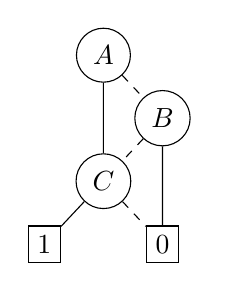
\begin{tikzpicture}[level distance=0.8cm]
      \node[draw,circle] (A) {$A$}
      child {edge from parent[draw=none]}
      child {node[draw,circle] (B) {$B$} edge from parent[dashed]
        child {node[draw,circle,solid] (C) {$C$} edge from parent[dashed]
          child {node[draw,rectangle,solid] {$1$} edge from parent[solid]}
          child {node[draw,rectangle,solid] (0) {$0$}}
        }
        child {edge from parent[draw=none]}
      };
      \draw (A) -- (C);
      \draw (B) -- (0);
    \end{tikzpicture}
    \caption{(RO)BDD}
  \end{subfigure}
  \begin{subfigure}{0.30\textwidth}
    \centering
    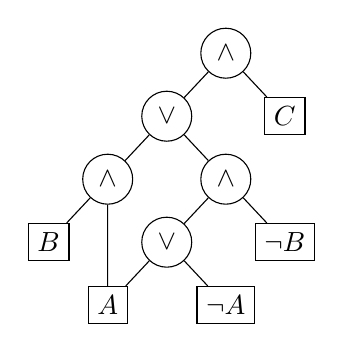
\begin{tikzpicture}[level distance=0.8cm]
      \node[draw,circle] {$\land$}
      child {node[draw,circle] {$\lor$}
        child {node[draw,circle] (parent) {$\land$}
          child {node[draw,rectangle] {$B$}}
          child {edge from parent[draw=none]}
        }
        child {node[draw,circle] {$\land$}
          child {node[draw,circle] {$\lor$}
            child {node[draw,rectangle] (A) {$A$}}
            child {node[draw,rectangle] {$\neg A$}}
          }
          child {node[draw,rectangle] {$\neg B$}}
        }
      }
      child {node[draw,rectangle] {$C$}};
      \draw (parent) -- (A);
    \end{tikzpicture}
    \caption{d-DNNF}
  \end{subfigure}
  \begin{subfigure}{0.30\textwidth}
    \centering
    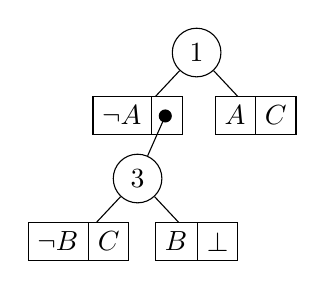
\begin{tikzpicture}[level distance=0.8cm]
      \tikzset{
        mysplit/.style={
          draw,
          rectangle,
          rectangle split,
          rectangle split horizontal,
          rectangle split parts=2
        }
      }
      \node[draw,circle] {$1$}
      child {node[mysplit] (bullet) {
          \nodepart{one} $\neg A$
          \nodepart{two}
        }
        child {node[draw,circle] (3) {$3$} edge from parent[draw=none]
          child {node[mysplit] {
              \nodepart{one} $\neg B$
              \nodepart{two} $C$
            }
          }
          child {node[mysplit] {
              \nodepart{one} $B$
              \nodepart{two} $\bot$
            }
          }
        }
      }
      child {node[mysplit] {
          \nodepart{one} $A$
          \nodepart{two} $C$
        }};
      \draw[*-] let \p1 = (bullet.two), \p2 = (bullet.center) in ({\x1 + 2.5},{\y2 + 2}) -- (3);
    \end{tikzpicture}
    \caption{SDD}
  \end{subfigure}
  \caption{Example diagrams for $C \land (A \lor \neg B)$}
\end{figure} % TODO: describe in text

\section{Progress To Date} \label{sec:progress}

\begin{figure}[t]
  \centering
  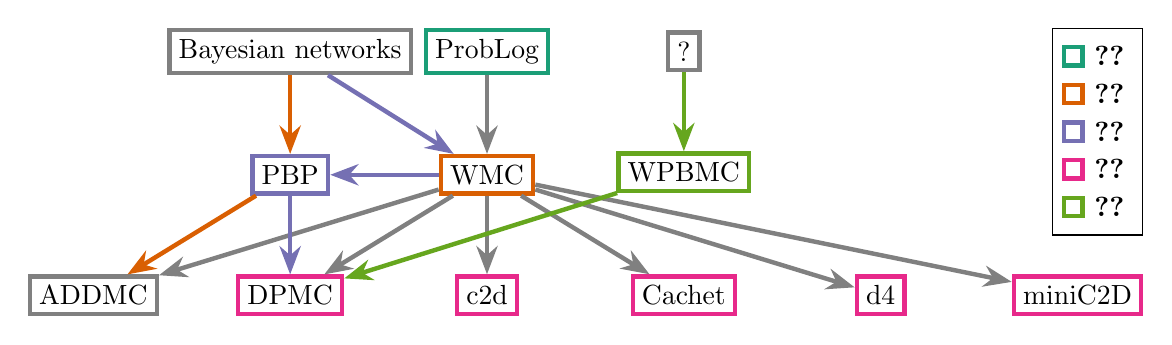
\begin{tikzpicture}[node distance=2.5cm]
    \node[draw,ultra thick,color=gray,text=black] (bn) {Bayesian networks};
    \node[draw,ultra thick,right of=bn,color=first,text=black] (problog) {ProbLog};
    \node[draw,ultra thick,color=gray,text=black,right of=problog] (unknown) {?};
    \node[draw,ultra thick,below=1cm of bn,color=third,text=black] (pbp) {PBP};
    \node[draw,ultra thick,below=1cm of problog,color=second,text=black] (wmc) {WMC};
    \node[draw,ultra thick,below=1cm of unknown,color=fifth,text=black] (wpbmc) {WPBMC};
    \node[draw,ultra thick,below=1cm of pbp,color=fourth,text=black] (dpmc) {DPMC};
    \node[draw,ultra thick,color=gray,text=black,left of=dpmc] (addmc) {ADDMC};
    \node[draw,ultra thick,right of=dpmc,color=fourth,text=black] (c2d) {c2d};
    \node[draw,ultra thick,right of=c2d,color=fourth,text=black] (cachet) {Cachet};
    \node[draw,ultra thick,right of=cachet,color=fourth,text=black] (d4) {d4};
    \node[draw,ultra thick,right of=d4,color=fourth,text=black] (minic2d) {miniC2D};
    \draw[-{Stealth},ultra thick,color=third] (bn) -- (wmc);
    \draw[-{Stealth},ultra thick,color=second] (bn) -- (pbp);
    \draw[-{Stealth},ultra thick,color=gray] (problog) -- (wmc);
    \draw[-{Stealth},ultra thick,color=third] (wmc) -- (pbp);
    \draw[-{Stealth},ultra thick,color=gray] (wmc) -- (addmc);
    \draw[-{Stealth},ultra thick,color=gray] (wmc) -- (dpmc);
    \draw[-{Stealth},ultra thick,color=gray] (wmc) -- (c2d);
    \draw[-{Stealth},ultra thick,color=gray] (wmc) -- (cachet);
    \draw[-{Stealth},ultra thick,color=gray] (wmc) -- (d4);
    \draw[-{Stealth},ultra thick,color=gray] (wmc) -- (minic2d);
    \draw[-{Stealth},ultra thick,color=second] (pbp) -- (addmc);
    \draw[-{Stealth},ultra thick,color=third] (pbp) -- (dpmc);
    \draw[-{Stealth},ultra thick,color=fifth] (unknown) -- (wpbmc);
    \draw[-{Stealth},ultra thick,color=fifth] (wpbmc) -- (dpmc);
    \matrix[draw,below left] at (current bounding box.north east) {
      \node[draw,color=first,ultra thick,label=right:\cref{app:cp}] {}; \\
      \node[draw,color=second,ultra thick,label=right:\cref{app:uai}] {}; \\
      \node[draw,color=third,ultra thick,label=right:\cref{app:sat}] {}; \\
      \node[draw,color=fourth,ultra thick,label=right:\cref{sec:1}] {}; \\
      \node[draw,color=fifth,ultra thick,label=right:\cref{sec:2}] {}; \\
    };
  \end{tikzpicture}
  \caption{Outline of concepts relevant to my past and future work. The first
    row contains representations of probability distributions that are and have
    been relevant to my work. The second row contains encodings, i.e.,
    computational problems that encode probabilistic inference. The third row
    contains WMC algorithms. The question mark denotes a representation that is
    yet to be identified. Gray arrows and boxes denote connections and concepts
    that are already known from previous work. A coloured arrow or box indicates
    that my work relates to that concept or interaction of concepts, and the
    colour coding describes which past or future paper the concept is related
    to.}
\end{figure} % TODO: describe in text

In this section, the progress made throughout this academic year is described
with respect to the work plan from my first year review.\footnote{The first year
review (with its own appendices) is included as \cref{app:previous}.}

\begin{description}
\item[WP 1] (`On the Equivalence of Constants in Relational Knowledge Bases')
  was abandoned. While trying to take reviewer feedback into consideration as
  well as update and strengthen the paper, I found an important ambiguity: when
  defining what constants are `captured' and `transferred' by a clause, I fail
  to specify whether each relevant `spot' is occupied by a constant or a
  variable. In the former case, that makes the main theorem of the paper
  completely trivial. While in the latter case, the theorem becomes incorrect. I
  spent a couple of weeks looking for ways to transform the paper into something
  both correct and valuable. The best idea I could find was to use the
  perspective from this paper in the context of inductive logic programming;
  however, I did not want to explore this direction further.
\item[WP 2] (`Generating Random Logic Programs Using Constraint
  Programming') was revised to include an experimental comparison of ProbLog
  inference algorithms and published and presented in CP~2020 (see \cref{app:cp}
  for the camera-ready version). I also gave three more talks about it:
  \begin{itemize}
  \item at the local AIAI seminar,
  \item for the Formal Analysis, Theory and Algorithms research section at the
    University of Glasgow,
  \item and at the FMAI~2021 workshop.
  \end{itemize}
\item[WP 3] was completed in full, although the emphasis shifted more towards
  experimental results than theory. It was first (unsuccessfully) submitted to
  AAAI~2021. Based on reviewer feedback, I updated the experimental section to
  compare not just various encodings with the same algorithm but also all of the
  encodings with the algorithms used in the original papers. The updated version
  can be found in \cref{app:uai} and was submitted to UAI~2021. I was also
  invited to the program committee for this conference.
\item[WP 4] was abandoned due to lack of contributions that could be made.
  Indeed, any contribution would have to be theoretical, empirical, or
  interpretability-related. Significant theoretical contributions are unlikely
  because the theory of abstractions has already been explored before without
  leaving behind any big unanswered questions \cite{DBLP:journals/kbs/Belle20}.
  While previous work could be rephrased in a simpler way and extended with more
  detail, the contributions would still be marginal.

  Furthermore, considering abstractions at their full level of generality is
  unlikely to be a viable method for improving inference speed because any
  abstraction is likely to be more computationally expensive than inference.
  Moreover, previous work on preprocessing for WMC left the field in an
  uncomfortable situation: preprocessing techniques for WMC were identified and
  described in a paper \cite{DBLP:conf/aaai/LagniezM14} whose main focus is on
  model counting; and the closed-source implementation of those techniques is
  unsuitable for WMC.

  Finally, a substantial issue with considering abstraction as a tool for
  interpretability---especially in the context of probabilistic relational
  models---is that the low-level building blocks such as predicate and constant
  names are usually semantically meaningful. Thus, replacing such a model with a
  simpler alternative that instead uses high-level concepts that are unlikely to
  correspond to words in any natural language is unlikely to improve
  interpretability despite the potential simplicity of this type of abstraction.
\item Furthermore, a new paper (not covered in the previous annual report) was
  written and submitted to SAT~2021 (see \cref{app:sat}). It originated as an
  attempt to improve \textbf{WP 3}: while the experimental results were
  impressive in the initial version of the paper, adding other algorithms
  revealed that instead of improving the state of the art by two orders of
  magnitude as originally thought, the suggested encoding was only fixing an
  underperforming algorithm and making its performance in line with other
  algorithms. The algorithm used for these experiments (ADDMC) was published
  only last year \cite{DBLP:conf/aaai/DudekPV20} and its experimental study
  includes some of the data used in my experiments as well as some new
  instances---one has to wonder whether the latter were added to improve the
  algorithm's comparative performance.

  First, my new paper replaces the previously used algorithm with its even newer
  version DPMC \cite{DBLP:conf/cp/DudekPV20}. The main improvement over ADDMC
  comes from the use of approximately-minimal-treewidth tree decompositions
  instead of heuristics for planning the order of multiplication and projection
  operations. After checking that DPMC performs very similarly with all
  encodings (including my own) and similarly to other WMC algorithms, the need
  to shift the contribution of my paper elsewhere became apparent.

  The main advantage of the encoding I proposed earlier was that it avoided
  parameter variables---something I claimed is completely unnecessary at
  least in WMC algorithms based on algebraic decision diagrams (ADDs) (i.e., a
  representation of pseudo-Boolean functions). However, the encoding was
  particularly rigid in that it always compiled each conditional probability
  table (CPT) in a Bayesian network into an ADD before doing anything else.
  Although this resulted in great inference speed improvements on some
  instances, e.g., when most of the probabilities in a CPT are equal, there is
  no reason to believe that such an approach is always optimal. Being unable to
  suggest a new encoding that clearly outperforms others, I decided to
  investigate how parameter variables could be removed from already-existing
  encodings. This led to a generalisation of WMC based on pseudo-Boolean
  functions that I named pseudo-Boolean projection (PBP). I then show how any
  WMC instance can be transformed into a PBP instance and identify conditions
  under which such a transformation can remove parameter variables. This
  transformation is applicable to four out of the five WMC encodings for
  Bayesian networks. Finally, experiments showed that (at least for some
  encodings) parameter variable removal can significantly improve inference
  speed and supersede the previous state of the art.
\end{description}

\section{Future Goals} \label{sec:future}

In this section, we describe two research projects to be completed before the
end of year 3. The first one is about \SI{30}{\percent} done at the time of
writing, while the second one is still just an idea with some notes. Note that
the total estimated duration for these projects leaves sufficient time for
thesis writing and potential unexpected delays in line with the plan from last
year.

\subsection{Parameterized Complexity of WMC in Theory and
  Practice} \label{sec:1}

The experiments in my papers in \cref{app:uai,app:sat} as well as in previous
work by others \cite{DBLP:conf/aaai/DudekPV20,DBLP:conf/cp/DudekPV20}
demonstrate that the differences amongst WMC algorithms are poorly understood,
i.e., the algorithms perform very similarly overall, but with significant
differences on subsets of benchmark data. In other words, which algorithm is the
best depends entirely on who provides the data, and we have no idea what
properties of a WMC instance make it more suitable for a search-based,
a compilation-based, or an ADD-based approach. Therefore, the paper I am working
on now aims to:
\begin{itemize}
\item Establish the parameterized complexity of DPMC, showing that it scales
  worse (than other algorithms) with respect to the treewidth of the primal
  graph of the input propositional formula in conjunctive normal form (CNF) (we
  call this \emph{primal treewidth}).
\item Propose a new random model for CNF formulas that allows us to generate
  instances of varying primal treewidth and use it to experimentally show how
  the performance of WMC algorithms depends on various properties of the
  instance such as density, primal treewidth, and the proportion of literal
  weights that are particularly `simplifying', e.g., zero, one, and perhaps a
  half.
\end{itemize}

\paragraph{Estimated duration:} 3 months.

\paragraph{Risks and contingencies.} One risk that I have already encountered is
that having all of the following can lead to an infeasible amount of computation
time:
\begin{itemize}
\item a time limit that is both similar to the time limits used in other
  experimental studies and provides enough `space' for a growth curve to express
  itself,
\item enough different parameter values so that the plots look more like the
  beautiful and barely-pixelated plots of today (e.g.,
  \cite{DBLP:conf/cp/McCreeshPP19,DBLP:journals/jair/McCreeshPST18}) and less
  like my tiny experimental setup in \cref{app:cp},
\item enough different random instances for each combination of parameter values
  so that a reliable median can be observed despite high variance.
\end{itemize}
This risk has been addressed in two ways:
\begin{itemize}
\item The time limit was reduced to \SI{100}{\second} and could be reduced
  further (e.g., a similar paper uses only a \SI{10}{\second} time limit
  \cite{DBLP:conf/ijcai/DudekMV17}).
\item Instead of iterating over the values of all parameters in one big
  experiment, I split it into two smaller experiments where some variables are
  held constant and others are allowed to vary.
\end{itemize}
Another risk is that the experimental results may be unclear and/or not easily
explainable. However, as random WMC instance generation is a completely
unexplored area, even weird or imperfect results still count as valuable and
interesting. Moreover, any unexpected differences in the way the algorithms
perform on random and real data can always be likened to the equivalent
situation with SAT algorithms.

\subsection{Weighted Pseudo-Boolean Model Counting} \label{sec:2}

\Cref{app:uai} and partially \cref{app:sat} address one issue with the
traditional definition of WMC, i.e., that restricting weights to literals leads
to most measures being unrepresentable without the addition of more variables
and clauses. It would be thematic to end the thesis by addressing the other
issue: at least for solvers such as ADDMC \cite{DBLP:conf/aaai/DudekPV20} and
DPMC \cite{DBLP:conf/cp/DudekPV20}, there is no reason for a clause to be just a
clause, i.e., a disjunction of literals. Instead, it can be an arbitrary
pseudo-Boolean function. In \cref{app:sat}, I suggested that two-valued
pseudo-Boolean function are particularly convenient because they can be defined
with a formal equivalent of the statement `if formula $\phi$ is satisfied, then
the value is $p$, otherwise the value is $q$'. Moreover, there is no reason for
the formula to be propositional! Instead, we can consider \emph{pseudo-Boolean
  constraints}\footnote{Despite similar names, pseudo-Boolean constraints and
  pseudo-Boolean functions are not related!}, i.e., an intermediary between SAT
and constraint satisfaction problems that supports linear and multilinear
inequality constraints on logical variables that are interpreted as ones and
zeros. Perhaps one can even use these constraints to encode almost arbitrary
arithmetic constraints on integers.

Extending DPMC to support such constraints is unlikely to be difficult. The
challenge is in finding at least one suitable application. The kind of Bayesian
network encodings that I investigated in \cref{app:uai,app:sat} \emph{can}
benefit from this (as they have counting constraints) but only marginally since
each counting constraint is usually only applied to two or three variables.
There must be some domain where probabilistic (or some other kind of weighted)
inference is needed in the context of integer arithmetic, counting, or
knapsack-style constraints, but so far I was not able to find one.

\paragraph{Estimated duration:} 6 months.

\paragraph{Risks and contingencies.} If I am unable to find a good
application, I will instead use the remaining time to work on a different idea,
e.g., adapting DPMC to first-order logic (i.e., WFOMC) using first-order ADDs
\cite{DBLP:journals/ai/SannerB09}.

\bibliographystyle{acm}
\bibliography{review}

\includepdf[pages=-,pagecommand=\thispagestyle{plain},picturecommand*={%
  \put(70,750){%
    \parbox{\textwidth}{\pagenumbering{gobble}\appendix\section{Published Paper (CP 2020)}\label{app:cp}}
  }}]{../../published/random-logic-programs/paper/paper.pdf}
\includepdf[pages=-,pagecommand=\thispagestyle{plain},picturecommand*={%
  \put(70,750){%
    \parbox{\textwidth}{\section{Submitted Paper (AAAI 2021 and UAI 2021)}\label{app:uai}}
  }}]{../../conditional-wmc/doc/paper2/paper.pdf}
\includepdf[pages=-,pagecommand=\thispagestyle{plain},picturecommand*={%
  \put(70,750){%
    \parbox{\textwidth}{\section{Submitted Paper (SAT 2021)}\label{app:sat}}
  }}]{../../conditional-wmc/doc/paper3/paper.pdf}
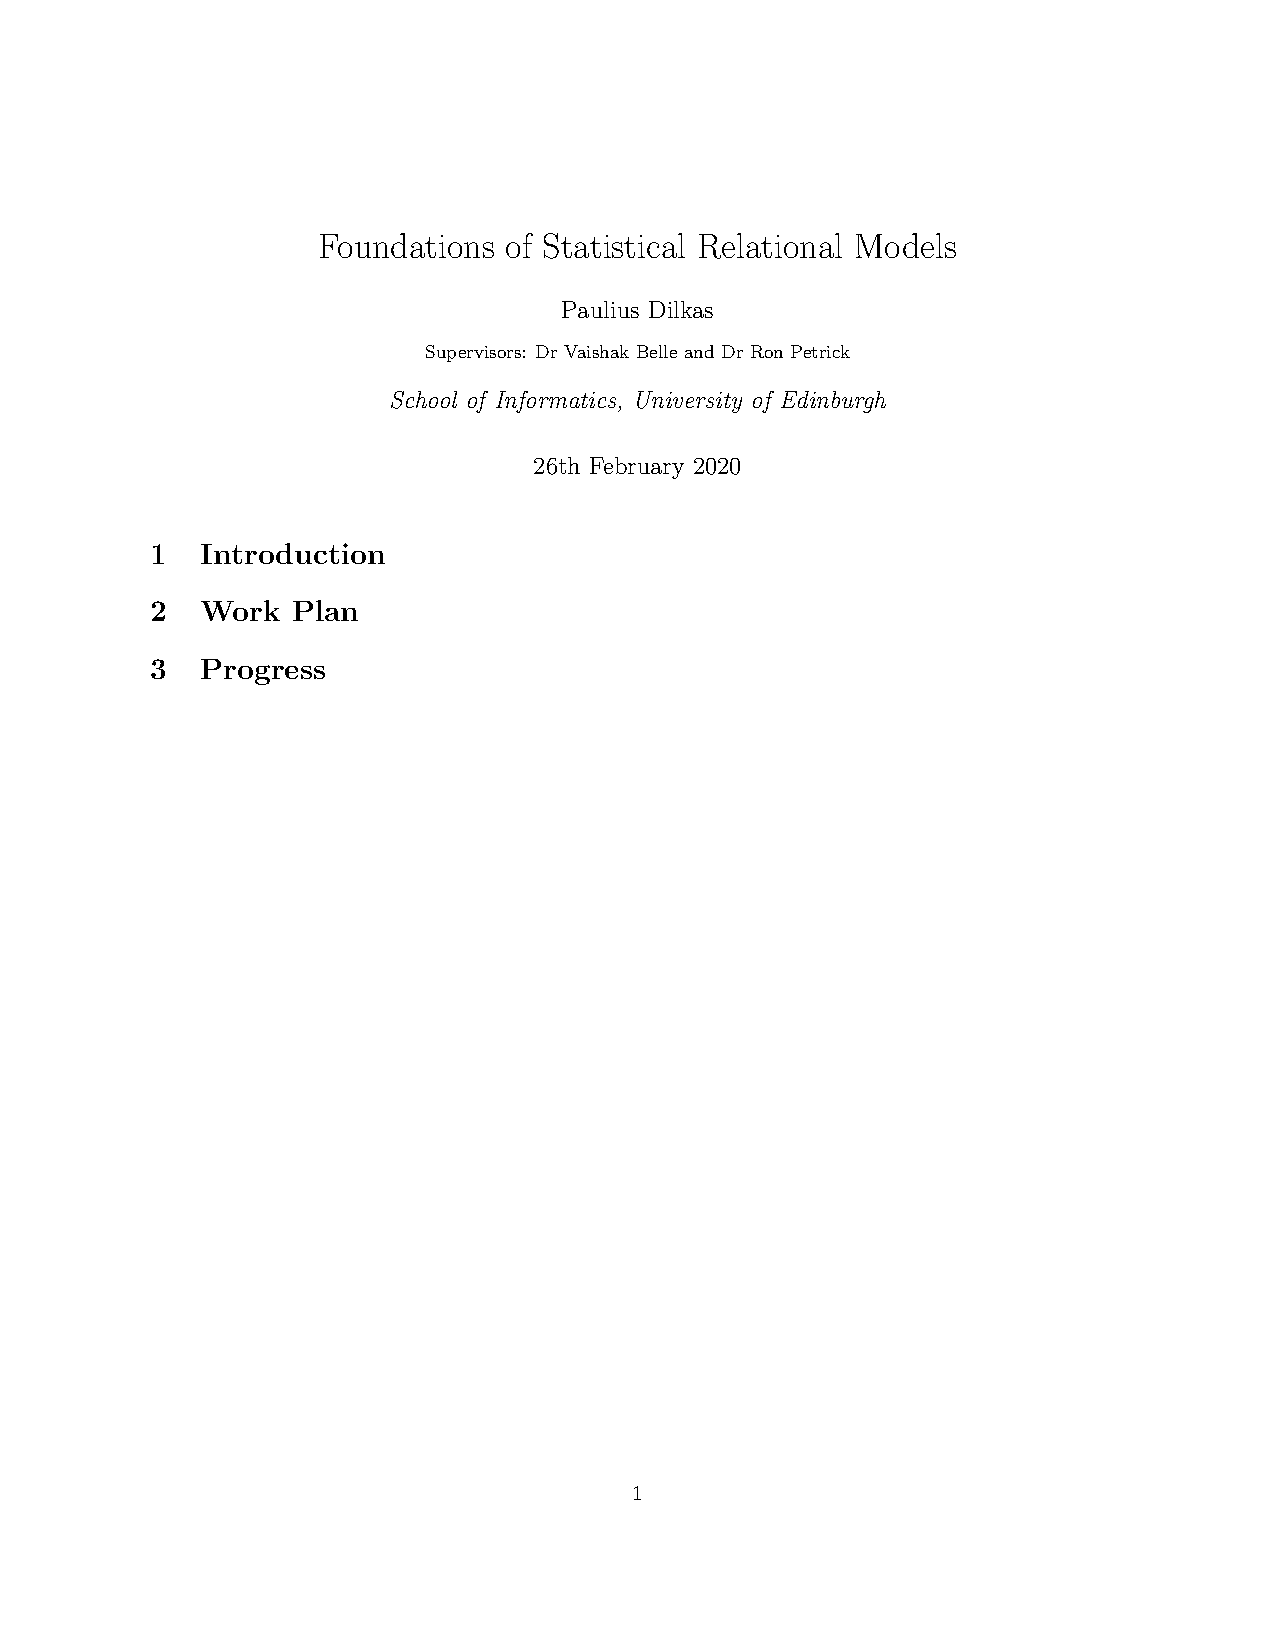
\includepdf[pages=-,pagecommand=\thispagestyle{plain},picturecommand*={%
  \put(70,750){%
    \parbox{\textwidth}{\section{First Year Review}\label{app:previous}}
  }}]{../review1/review.pdf}

\end{document}